\documentclass[article, a2paper, oneside, landscape]{memoir}
\usepackage{tikz,tree}
\usetikzlibrary{mindmap}
\pagestyle{empty}

\begin{document}
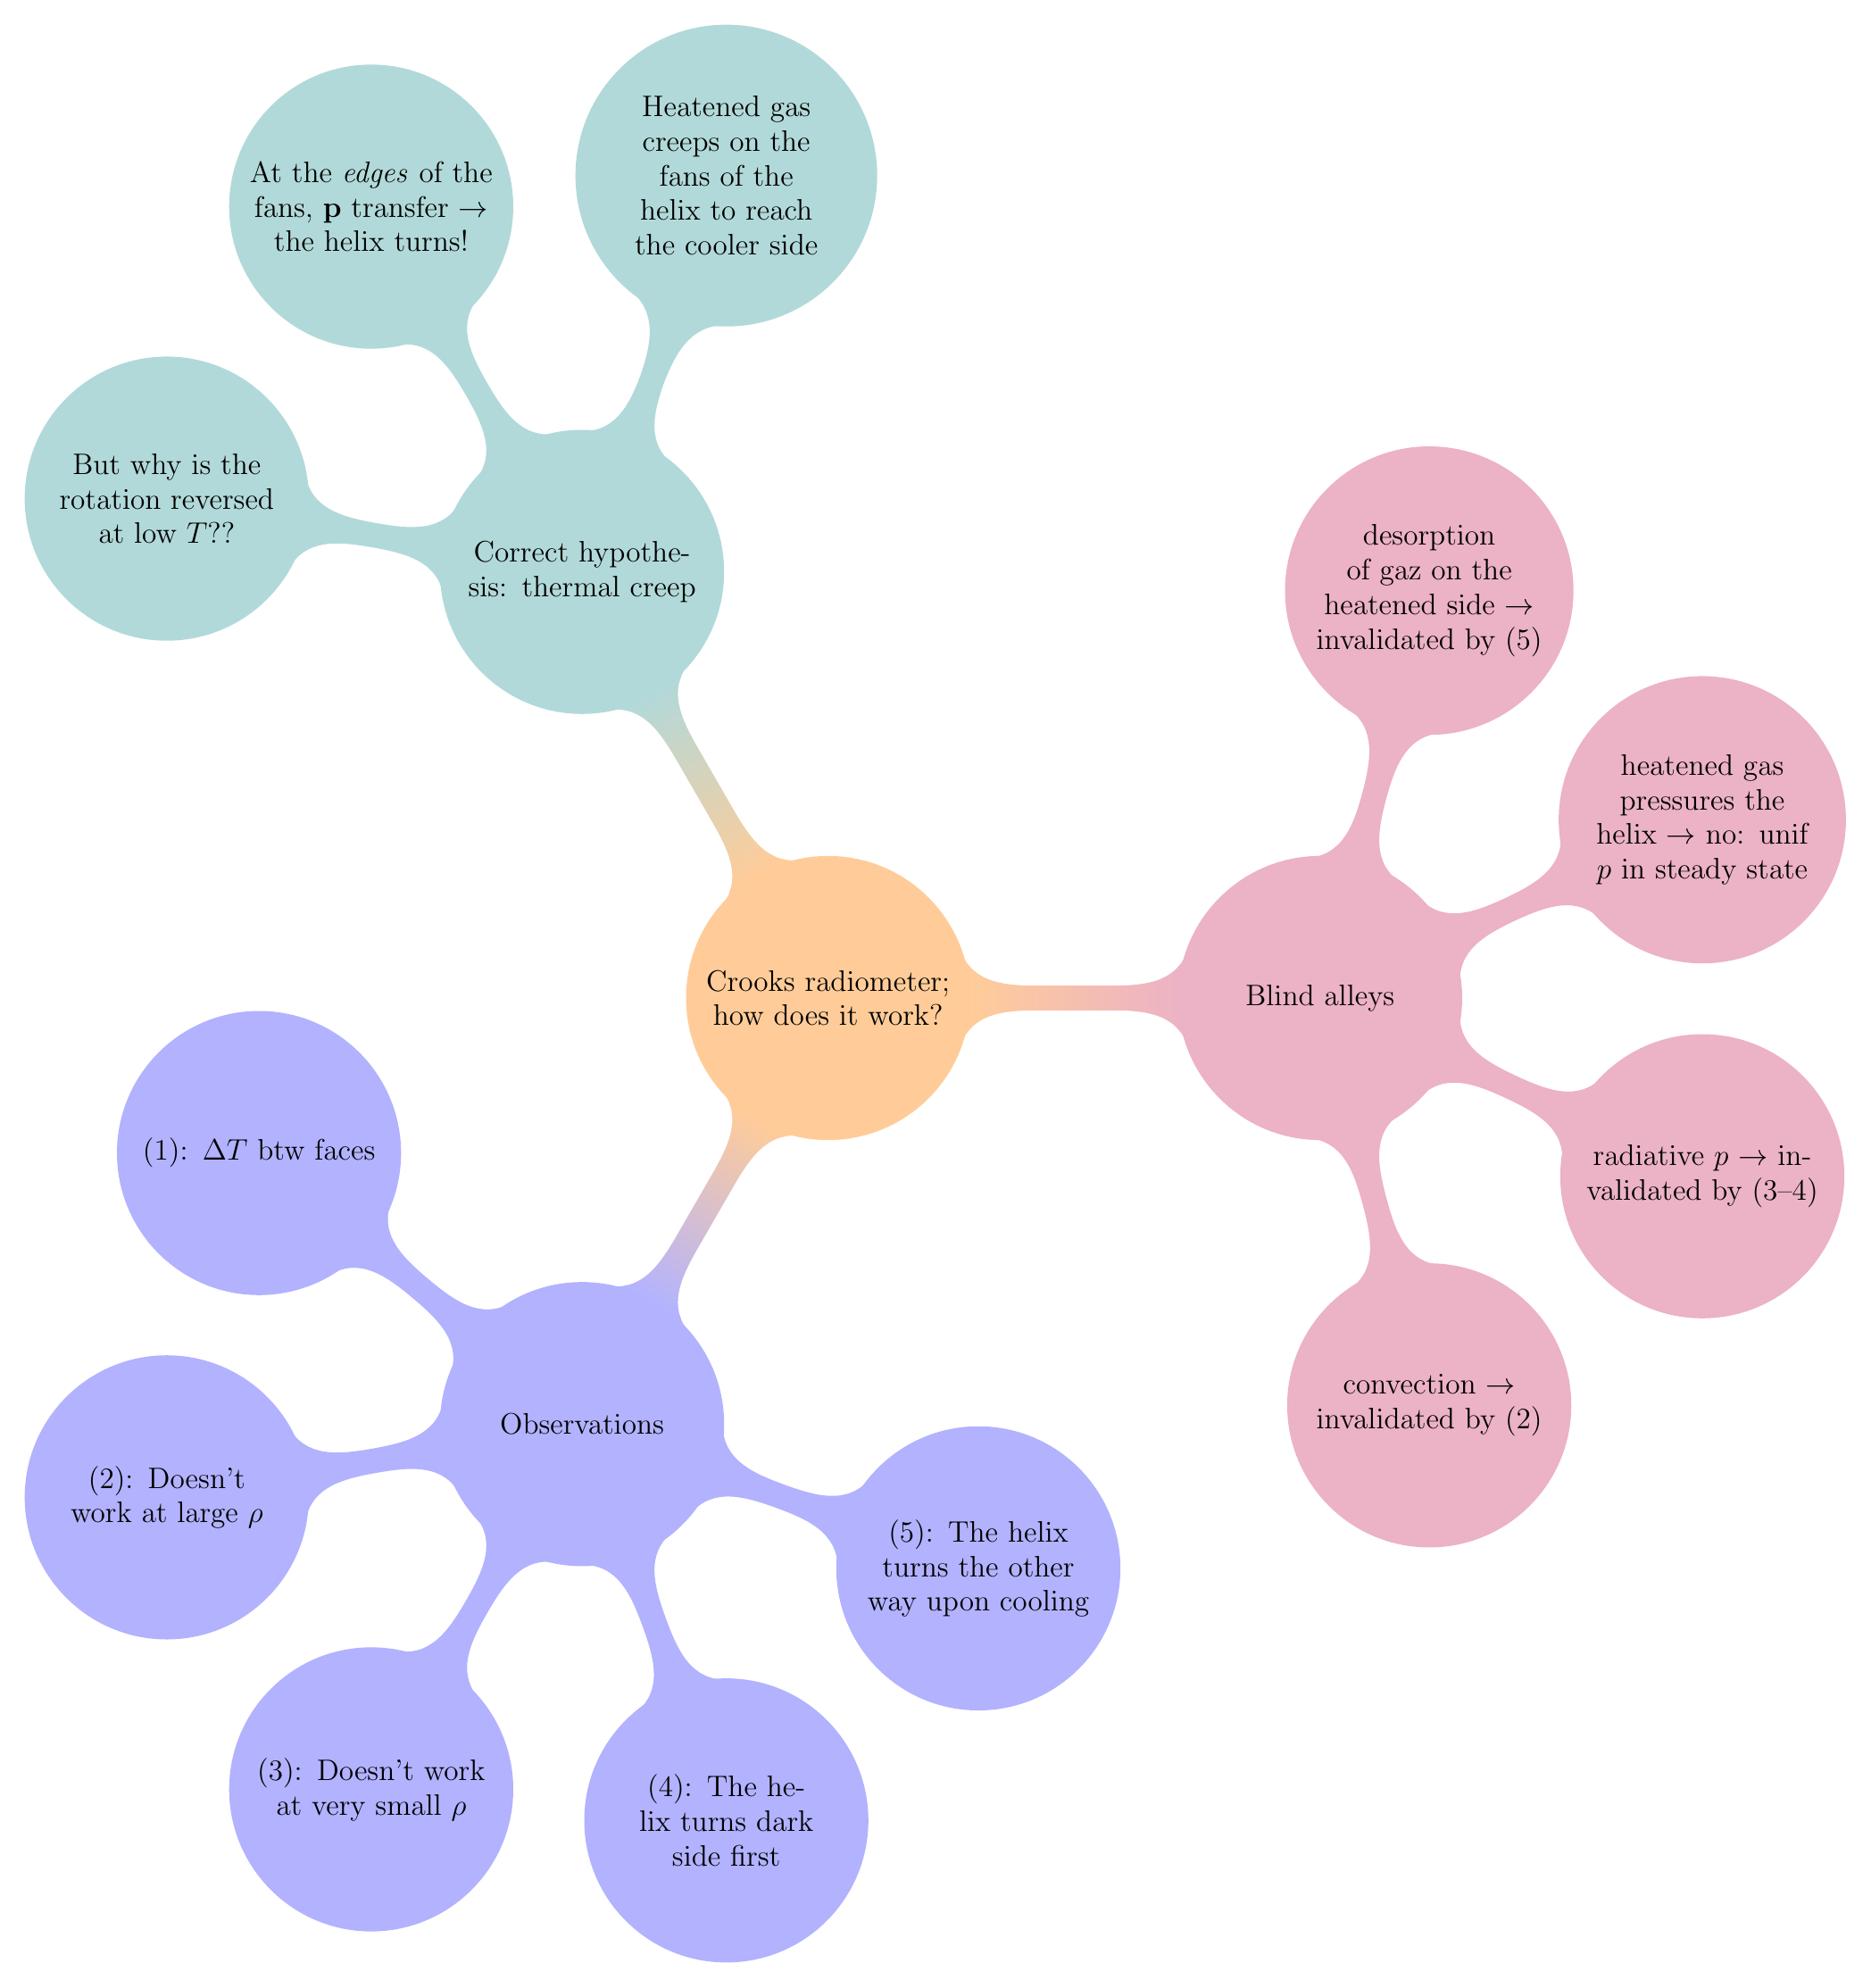
\begin{tikzpicture}[mindmap, grow cyclic, every node/.style=concept, concept color=orange!40,
  level 1/.style={level distance=7cm,sibling angle=120},
  level 2/.style={level distance=6cm,sibling angle=50},
  level 3/.style={level distance=6cm,sibling angle=90}]

\node{Crooks radiometer; how does it work?}
  child [concept color=blue!30] { node {Observations}
      child { node {(1): $\Delta T$ btw faces}}
      child { node {(2): Doesn't work at large $\rho$}}
      child { node {(3): Doesn't work at very small $\rho$}}
      child { node {(4): The helix turns dark side first}}
      child { node {(5): The helix turns the other way upon cooling}}
  }
  child [concept color=purple!30] { node {Blind alleys}
    child { node {convection $\rightarrow$ invalidated by (2)}}
    child { node {radiative $p$ $\rightarrow$ invalidated by (3--4)}}
    child { node {heatened gas pressures the helix $\rightarrow$ no: unif $p$ in steady state}}
    child { node {desorption of gaz on the heatened side $\rightarrow$ invalidated by (5)}}
  }
  child [concept color=teal!30] { node {Correct hypothesis: thermal creep}
    child { node {Heatened gas creeps on the fans of the helix to reach the cooler side}}
    child { node {At the \emph{edges} of the fans, $\mathbf{p}$ transfer $\rightarrow$ the helix turns!}}
    child { node {But why is the rotation reversed at low $T$??}}
  }
;

\end{tikzpicture}
\end{document}
